\documentclass[tikz,border=7pt]{standalone}
\begin{document}
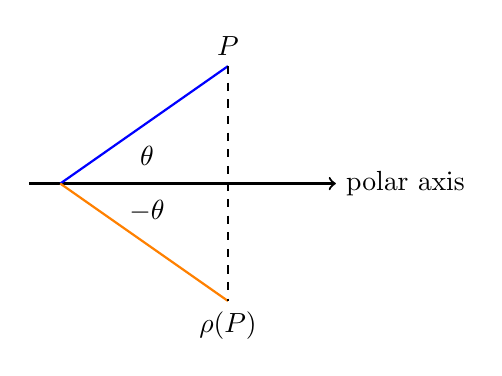
\begin{tikzpicture}[line width=.8pt]
\draw[->] (-.4,0)--(3.5,0) node[right] {polar axis};
\draw[blue,thick] (0,0)--(35:2.6); \draw[orange,thick] (0,0)--(-35:2.6);
\draw[dashed] (35:2.6)--(-35:2.6);
\node[above] at (35:2.6) {$P$}; \node[below] at (-35:2.6) {$\rho(P)$};
\node at (1.1,.35) {$\theta$}; \node at (1.1,-.35) {$-\theta$};
\end{tikzpicture}
\end{document}
